\chapter{Motivation}
\label{chap:motivation}
The initial version of the learning environment (LDBN) was used in
conjunction with the course \emph{Principles of Database Systems} at the 
Department of Computing Science at Ume� University, and some important 
observations were made. In this chapter we present the problems with the 
initial version of LDBN, which were observed during this testing period. 
Some of the problems let us realized that LDBN needs to be further developed 
%ne mi haresva
and extended in order for all users to make a more extensive and productive use 
of the system, and in order for the students to be assisted even better 
in the process of understanding the concepts of FDs and 
relational-database normalization by providing new tools to them such as the 
FD visualization tool, which is described in detail in Section~\ref{sec:visualization}.  

\section{Problem Statement}
\label{sec:problem_statement}
At the moment, students, who are trying to solve an assignment with LDBN, often have
to deal with a large number of attributes and FDs based on those attributes. 
However, LDBN offers only textual representation of FDs, an example of such
representation is shown in Figure~\ref{fig:exampleFds01} . 

\begin{figure}[h]
	\begin{center}
		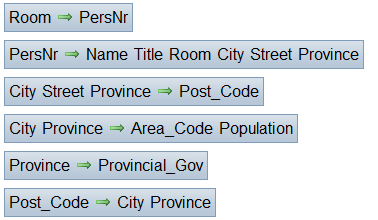
\includegraphics[width=0.7\textwidth]{./img/example_fds_01.png}
		\caption{Example of a Typical Textual Representation of FDs}
		\label{fig:exampleFds01}
	\end{center}
\end{figure}


As it can be seen, some attributes 
may occur more than once in a single FD and there could be many different FDs in a single 
assignment. Although this is a standard representation of FDs, 
it could lead to a confusion among students and negatively affect the overall
usability of the system. Thus we extended LDBN by providing a visualization for
FDs. In order the visualization to be intuitive for 
both students and lecturers we have decided to use templates found in popular 
popular database textbooks such as~\cite{bdb2} and~\cite{bdb1}. 
Example of a such visualization can be observed in Figure~\ref{fig:viz-fds-ex01}.

\begin{figure}[h]
	\begin{center}
		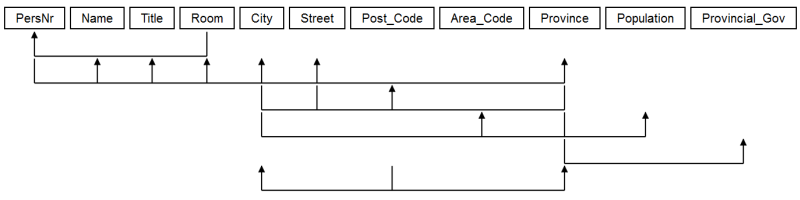
\includegraphics[width=0.95\textwidth]{./img/viz-fds-ex01.png}
		\caption{Example of a Graphical Representation of FDs}
		\label{fig:viz-fds-ex01}
	\end{center}
\end{figure}

Another major problem with the initial system is the fact that all 
registered users have the same rights. Thus all users can create assignments, which
can be seen by all other registered or unregistered users. In addition, assignments
can be viewed in the \emph{Solve Assignment Tab} only if they have been previously
stored in the system by a registered user. In the original version of LDBN,
it was believed that both of these facts would increase the number and the diversity of
assignments stored in the systems, and thus the system would appeal to more students 
and increase usability. 
This collaborative approach has been inspired by the Wikipedia project, where everyone
can be a content contributor and a reader at the same time. 
However, during the testing period the system has been flooded with unsuitable assignments
mainly because of two reasons. First, 
identical assignments occurred more than once under different names. They were usually submitted 
by students in the same class trying to
solve a homework assignment, or just trying the system with examples from textbooks.
Second, users were unable to load an assignment in the \emph{Solve Assignment Tab}
without first storing it in the database of the system, this led to the fact that
users who just wanted to test the system with a simple assignment, were in fact
flooding LDBN with even more unsuitable assignments, which consist of just a 
few arguments and even less FDs and were of no interest to other users. Both of these
facts led to a major decrease in the usability of the system, 
since students were no longer able to distinguish 
between interesting and well-thought-out assignments submitted by lecturers 
and other assignments.
 
To solve the above problem a more sophisticated user system was introduced. In the 
current version of LDBN users are basically dividend into two groups - 
regular users (students) and administrators (lecturers).
First, administrators 
have more rights than regular users. Second, only assignments submitted by administrators
are visible by default.  
In addition, lecturers have much more rights in the system than students.
This is discussed in detail in Section~\ref{sec:improving}. 
 

\section{Purpose}
\label{sec:purpose}
The purpose of this thesis can be divided into two parts:

\begin{enumerate}

  \item Implementing different types of visualization for FDs based 
  on templates found in popular textbooks such as~\cite{bdb2} and~\cite{bdb1}. 
  Furthermore, the visualization should support different colors schemata and 
  zoom levels for a better presentation. In addition to this, the visualization
  should be available for all fields in the UI which hold a set of FDs and it should
  not interfere with existing representation of the FDs.

  \item Improving the existing system in several ways including:
  
  \begin{enumerate}
    \item Dividing the user into at least two groups: 
    (1) administrators and (2) regular registered users. This is done without
    affecting the existing users, thus all already registered users will keep
    their rights in the system. 
    \item Decrease the number arbitrary assignments by providing new methods for saving and 
    loading assignments in the system. 
    \item User should be able to delete and edit their previously submitted comments.    
  \end{enumerate}
  
\end{enumerate}

%TODO some more motivation so you can get four pages for this chapter
 